\documentclass{article}
\usepackage[T2A]{fontenc}
\usepackage[utf8]{inputenc}
\usepackage[english,russian]{babel}
\usepackage{enumitem}
\usepackage{multicol}
\usepackage{ulem}
\usepackage{graphicx}
\usepackage{geometry}
\geometry{left=20mm, right=20mm, top=17mm, bottom=9mm, nohead, nofoot}
\setcounter{page}{233}
\begin{document}
\begin{multicols}{2}
Also in [28] examples of knowledge extraction,
\uline{entities from Wikipedia articles} are discussed. Wikipedia
data uses the MediaWiki API to extract article and category content and metadata from Wikipedia. An article
can be specified as a string or Wolfram Language object.
Retrieving articles associated with language entities is
provided by the WM TextSentences feature, in particular, it is possible to work with Wikipedia resources.
Presented are specific results of the TextSentences function, with parameters WikipediaData, Entity, “Person”,
“AlexeiLeonov”.

These examples of working with knowledge bases
using WM tools, since the system kernel functions can be
used in programs developed on other platforms, can be
interpreted as proposals for the innovative improvement
of existing tools, components of any intelligent computer
systems, and of course the Ecosystem OSTIS.

\begin{center}
VI. EXAMPLE OF INTEGRATING WOLFRAM
MATHEMATICA WITH EDUCATIONAL OSTIS-SYSTEM
PROTOTYPE FOR DISCIPLINE “COMPUTER SYSTEMS
AND NETWORKS”
\end{center}
Here is an illustration of the combined use of WM and
OSTIS-prototype for discipline “Computer Systems and
Networks” ostis-system for working with computer network topologies. The results below show the possibilities
of using the visualization performed in WM in the ostissystem. Moreover, implementations are available using
an appropriate programming interface (it is possible to
execute WL code hosted in the Wolfram cloud within a
user program, such as Python or C++ [29]) or import, export tools. According to Mathematica $\uline{ImportFormats}
and $\uline{ExportFormats} functions, it supports more than
100 formats, the list of formats is as follows:

3DS, ACO, Affymetrix, AgilentMicroarray, AIFF,
ApacheLog, ArcGRID, AU, AVI, Base64, BDF, Binary, Bit, BMP, BSON, Byte, BYU, BZIP2, CDED,
CDF, Character16, Character8, CIF, Complex128, Complex256, Complex64, CSV, CUR, DAE, DBF, DICOM,
DIF, DIMACS, Directory, DOT, DXF, EDF, EML,
EPS, ExpressionJSON, ExpressionML, FASTA, FASTQ,
FCS, FITS, FLAC, GenBank, GeoJSON, GeoTIFF, GIF,
GPX, Graph6, Graphlet, GraphML, GRIB, GTOPO30,
GXL, GZIP, HarwellBoeing, HDF, HDF5, HIN, HTML,
HTTPRequest, HTTPResponse, ICC, ICNS, ICO, ICS,
Ini, Integer128, Integer16, Integer24, Integer32, Integer64, Integer8, JavaProperties, JavaScriptExpression,
JCAMP-DX, JPEG, JPEG2000, JSON, JVX, KML, LaTeX, LEDA, List, LWO, M4A, MAT, MathML, MBOX,
MCTT, MDB, MESH, MGF, MIDI, MMCIF, MO,
MOL, MOL2, MP3, MPS, MTP, MTX, MX, MXNet,
NASACDF, NB, NDK, NetCDF, NEXUS, NOFF, OBJ,
ODS, OFF, OGG, OpenEXR, Package, Pajek, PBM,
PCAP, PCX, PDB, PDF, PGM, PHPIni, PLY, PNG,
PNM, PPM, PXR, PythonExpression, QuickTime, Raw,

\noindent RawBitmap, RawJSON, Real128, Real32, Real64, RIB,
RLE, RSS, RTF, SCT, SDF, SDTS, SDTSDEM, SFF,
SHP, SMA, SME, SMILES, SND, SP3, Sparse6, STL,
String, SurferGrid, SXC, Table, TAR, TerminatedString,
TeX, Text, TGA, TGF, TIFF, TIGER, TLE, TSV,
UBJSON, UnsignedInteger128, UnsignedInteger16, UnsignedInteger24, UnsignedInteger32, UnsignedInteger64,
UnsignedInteger8, USGSDEM, UUE, VCF, VCS, VTK,
WARC, WAV, Wave64, WDX, WebP, WLNet, WMLF,
WXF, XBM, XHTML, XHTMLMathML, XLS, XLSX,
XML, XPORT, XYZ, ZIP.

In the example below, the initial data (a particular
graph of the topology of a computer network) is imported
from a teaching ostis-system for the “Computer Systems
and Networks” discipline, visualized by WM graphics,
then solved the typical problem and the preferred final
results are exported back to the teaching ostis-system
for the discipline. Initial data, the specific graph of the
network topology used next is shown in the Fig. 2.

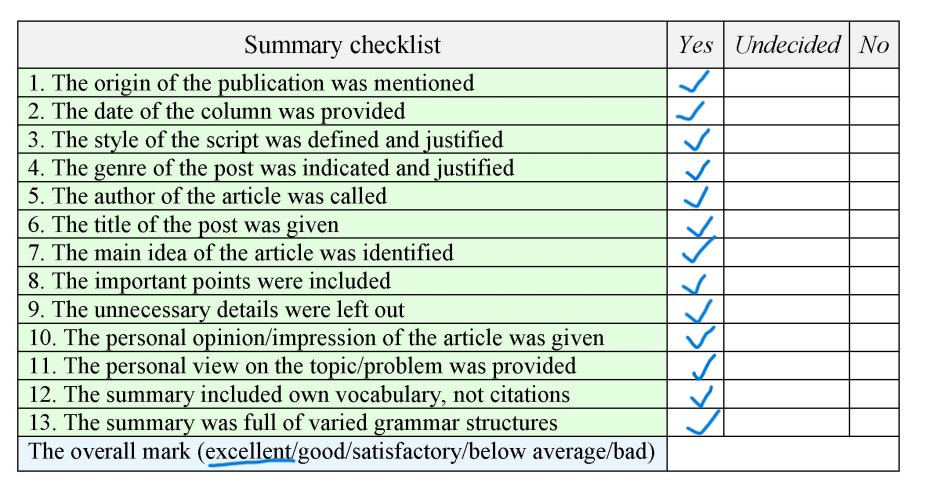
\includegraphics[width=80mm, height=70mm]{Screenshot_1.png}
{\fontsize{8pt}{12pt}\selectfont Figure 2. Network topology graph, nodes and connections (in the
ostis-system).}

The following illustrations are generated in WM.
For the imported graph in WM, you can get general
information such as: number of vertices (network nodes),
list of edges (connections between nodes), and visualize
it. Fig. 3 shows the output of the vertex list (VertexList),
the number of edges (EdgeCount), and the edges list
(EdgeList).

The three output layouts are shown below for an example visualization. Fig. 4 shows vertices and edges with
their weights. This form of representation is preferable
for visualization of logical network topology, in which
the directions of data flows are indicated. Edges with
\end{multicols}
\end{document}
